\section{支撑材料与程序索引}\label{appendix-start}
\subsection{目录与复现入口}
支撑材料包含本版论文对应的模型、原始资料、参数配置、保存的计算结果、图表生成代码及本稿源文件。源文件沿用实际调用所需的名称；目录中的编号用于标识计算核与结果来源。
\begin{table}[H]\centering\caption{本版支撑材料目录与入口}
\begin{tabularx}{\linewidth}{p{.20\linewidth}X}\toprule
目录或入口 & 内容与用途\\\midrule
\path{src/} & 年度模型、投资搜索、连续事件、约束核验和图文生成程序\\
\path{config/} & 模型参数、情景与固定实验配置\\
\path{data/} & 官方附件、原始资料与预处理数据\\
\path{simulation/} & MATLAB/Simulink与AnyMath原生模型、控制器和状态接口\\
\path{outputs/} & 本文计算结果、逐案状态、矩阵、配对表和求解记录\\
\path{figures/} & 当前图件的可编辑矢量文件\\
\path{paper/} & 本版论文TeX稿源与正文使用图件\\
\bottomrule\end{tabularx}\end{table}
\noindent\textbf{图表与论文：}\texttt{复现图表与论文.py}，读取随附结果、重绘图表并编译论文。\par
\noindent\textbf{MATLAB：}\path{start_v9_lab.m}，启动原生物理网络与交互实验台。\par
\noindent\textbf{AnyMath：}\path{simulation/anymath_v10/start_v10.jl}，启动原生小时滚动优化。\par

\subsection{原生状态连接与计算入口}\label{app:anymath-native}
MATLAB原生环境采用R2026a、Simulink及Optimization Toolbox，小时求解调用\texttt{linprog}。实验台聚焦折中2060快照：控制器提出动作，原生物理网络推进库存、SOC、债务和机组记忆；支持初始化、单步、24小时推进、连续与暂停。回放读取已执行完整轨迹并单独标识；改变原生输入后重新初始化。

\begin{figure}[H]\centering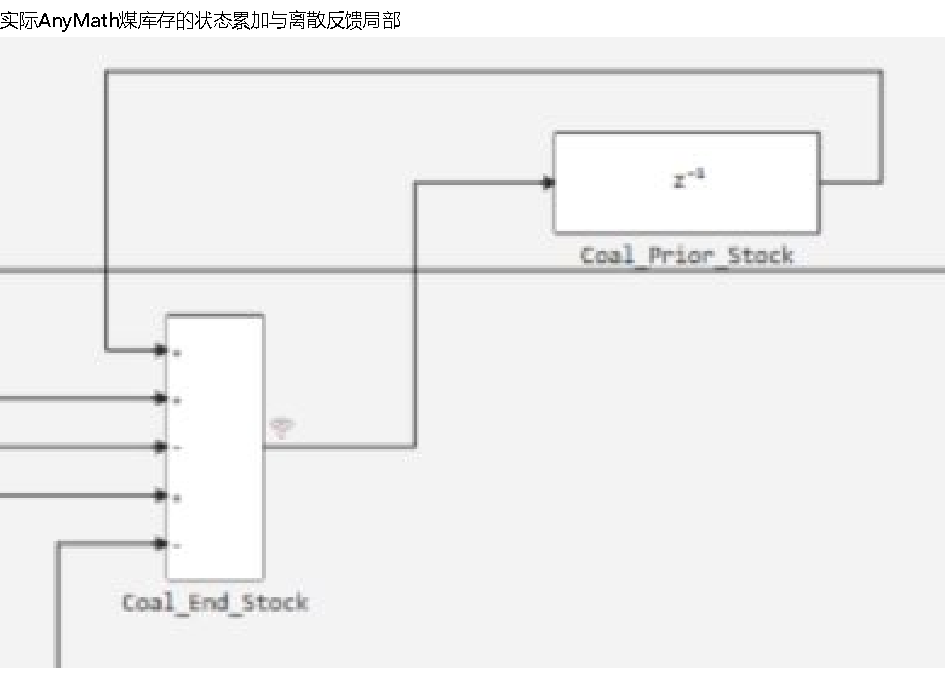
\includegraphics[width=\linewidth]{figures/native_anymath_state_feedback.pdf}\caption{实际平台截图的状态反馈局部。左侧信号进入Coal\_End\_Stock加和模块，更新库存经Coal\_Prior\_Stock离散延迟反馈到下一步。}\end{figure}

Python执行年度实验、可靠性投资搜索与连续事件计算，图表读取保存结果。年度与历史检验的对应程序为\path{src/v6_annual_experiments.py}，投资搜索程序为\path{src/v6_planning.py}，连续事件程序为\path{src/v6_resilience.py}。离线边界与守恒证据对应\path{src/v15_dispatch_bound_v2.py}和\path{src/v15_energy_cut_certificate.py}；联合约束、末态与数值表示核验对应\path{src/v16_joint_dispatch.py}、\path{src/v16_endpoint_peak.py}、\path{src/v16_endpoint_numerics.py}和\path{src/v16_endpoint_bound_form.py}。原始求解状态与失败记录和成功结果一并保留。

AnyMath每小时以上一实际末状态初始化原生记忆，在\texttt{StopTime=0}处求值一个隐含$\Delta t=1$ h的离散资源转移，返回8维末状态后继续优化；小时索引由外层会话推进。滚动LP存在多最优解，跨实现核验比较同状态最优目标与物理可行性，不要求首动作唯一。实际云执行含中断后从同版本、同8维末状态续算的路径，前缀与衔接核对保留在对应计算结果中。

\section{原生原型与最优解选择的补充图表}
\subsection{储能状态如何改变高峰时的实际交付}
实验台显示当前方案、供给方式、策略及实际已执行小时。原生模式支持初始化、单步、24小时推进、连续和暂停，曲线仅显示已求解前缀；保存轨迹回放使用独立标识。输入改变后重新初始化，避免把新参数套在旧状态上。
\begin{figure}[H]\centering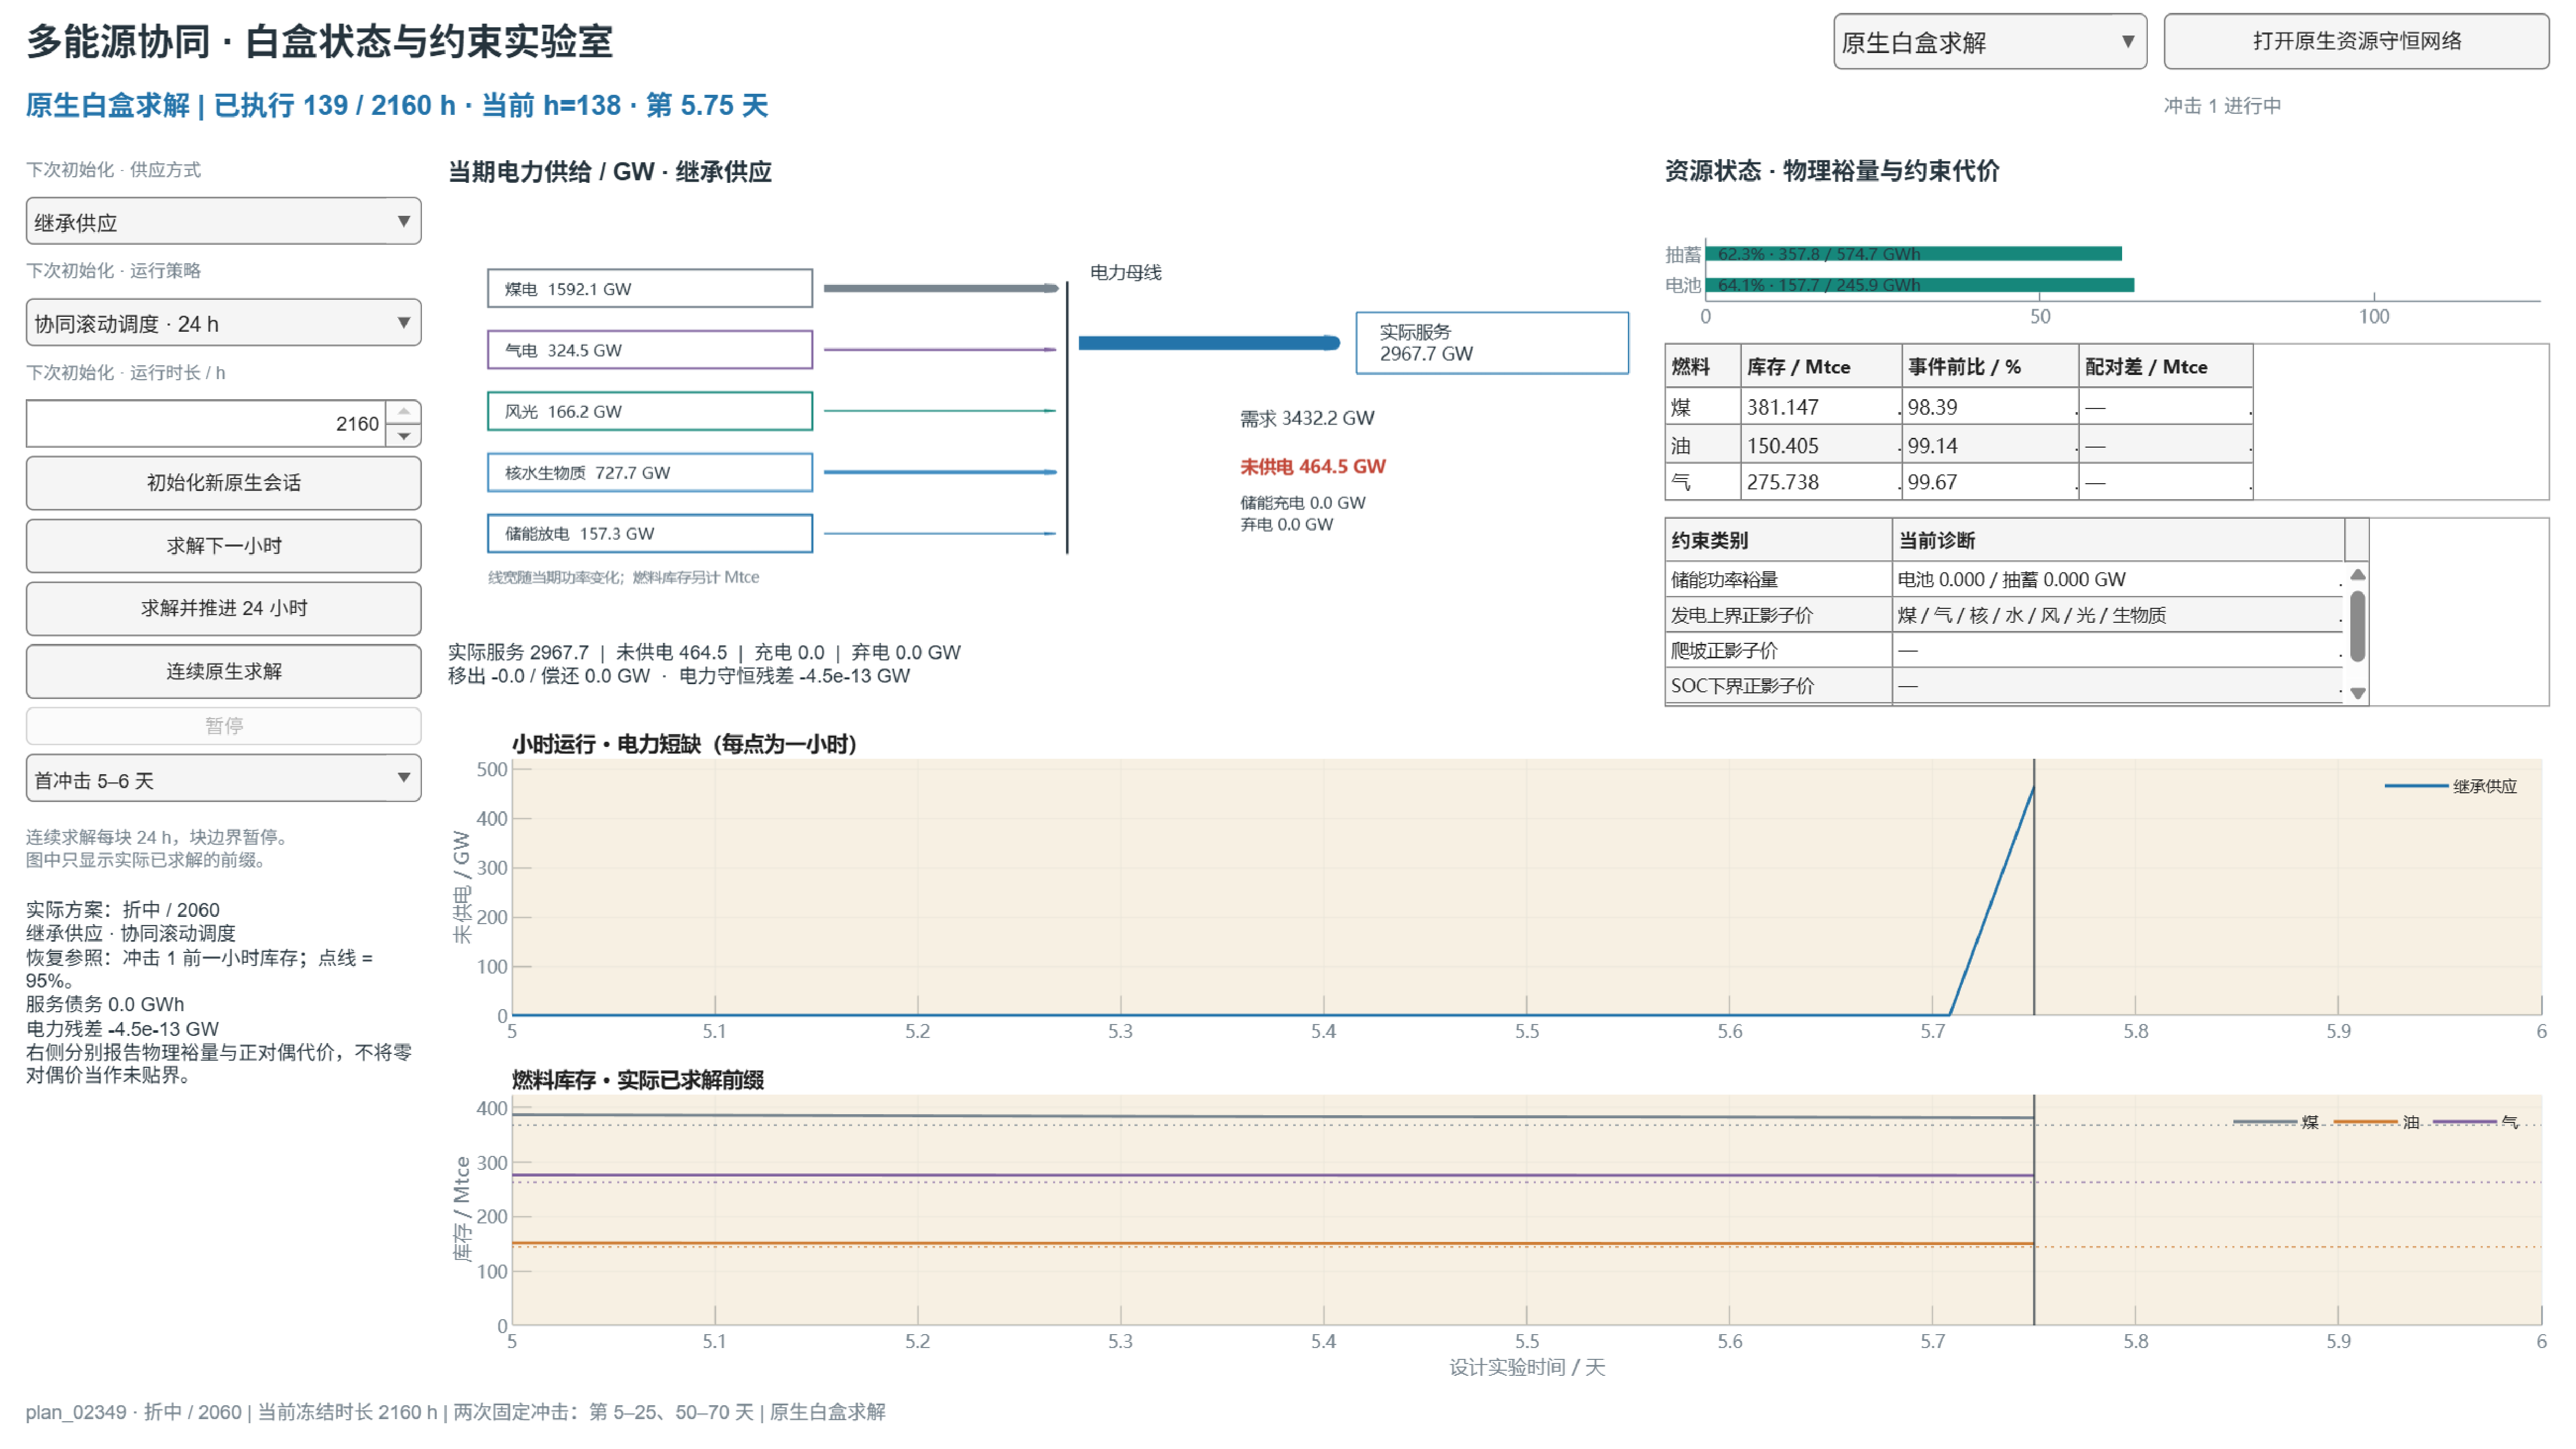
\includegraphics[width=160mm]{figures/native_v9_app_overview.pdf}\caption{实际原生求解至h=138的过程实验台。能流与库存对应同一小时，窗口同时显示已执行前缀、缺供和约束状态；该截图来自新物理资源网络。}\end{figure}

\begin{table}[H]\centering\caption{相同初态与外部输入下的两条原生状态路径}
\begin{tabular}{lrr}\toprule
状态或交付 & 协调 & 分散\\\midrule
h=137末电池SOC / GWh & 222.478 & 0.000 \\
h=137末抽蓄SOC / GWh & 466.240 & 0.000 \\
h=138电池放电 / GW & 61.487 & 0.000 \\
h=138抽蓄放电 / GW & 95.782 & 0.000 \\
h=138未供电 / GW & 464.457 & 621.726 \\
h=0--144累计未供电 / GWh & 1,530.829 & 2,271.709 \\
\bottomrule\end{tabular}\end{table}

第137小时末，协调路径仍保留电池与抽蓄能量，分散路径已耗尽。第138小时，两类储能合计交付157.269 GW，恰与两路径该小时的缺电差对应；截至第144小时，协调路径累计少缺供740.879 GWh。

将两种策略从\textbf{同一个第137小时末状态、同一未来24小时输入}重新分支，第138小时未供电均为464.457 GW，差值为零。因此，这一峰时的路径收益来自此前形成的储能状态，而非同状态下该时刻产生了更高的即时供电。此处聚焦协调与分散各145小时的状态路径；前述90天交付与库存结果，另由两种供应方式下各2160小时的完整原生运行核对。
\FloatBarrier


\begin{figure}[H]\centering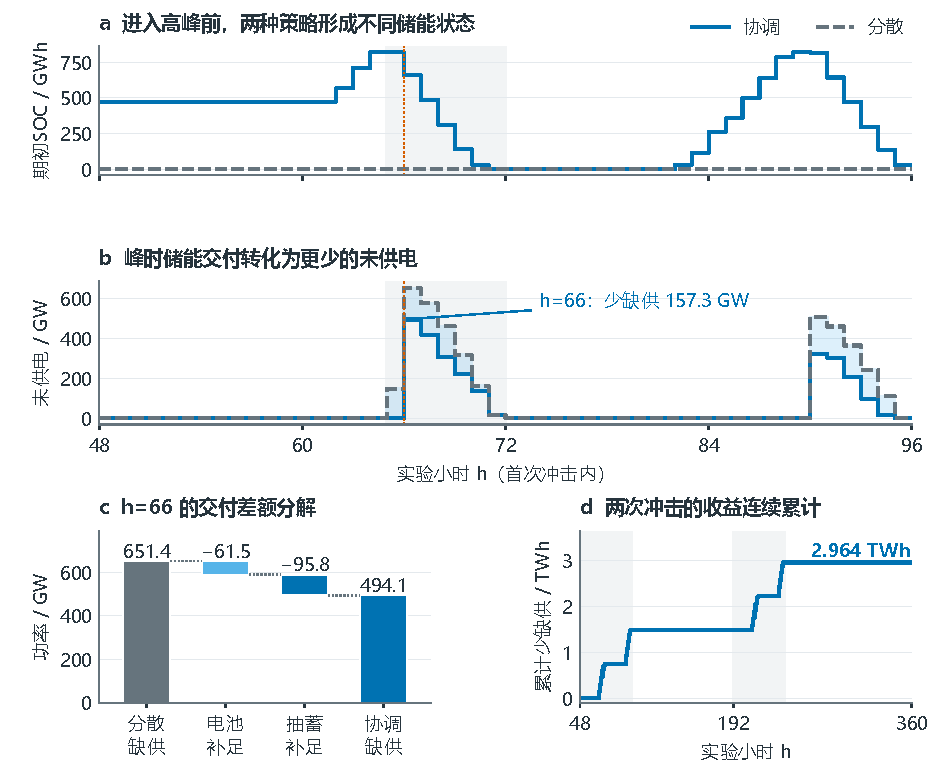
\includegraphics[width=\linewidth]{figures/figH_coordination_mechanism.pdf}
\caption{协调相对指定非化石局部规则的动作链：首次冲击内的逐小时期初SOC、峰值时储能交付及累计缺供。各面板读取相同已执行轨迹，收益统计统一为第48—359小时。}\label{fig:figH_coordination_mechanism}\end{figure}

\begin{figure}[H]\centering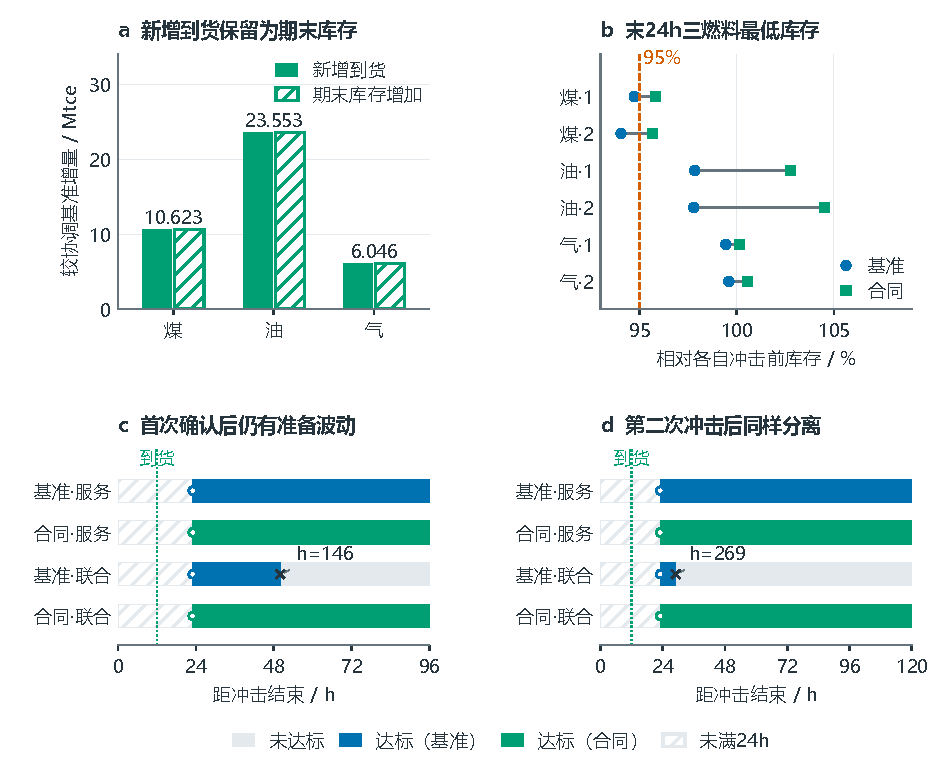
\includegraphics[width=\linewidth]{figures/figJ_contract_readiness.pdf}
\caption{合同到货如何形成资源准备。新增到货与末库存增量逐燃料核对；库存底线取事件边界前完整24小时内的最小比值，分母为各方案各事件的冲击前库存。色带分别表示服务窗口与联合准备窗口。}\label{fig:figJ_contract_readiness}\end{figure}

\begin{figure}[H]\centering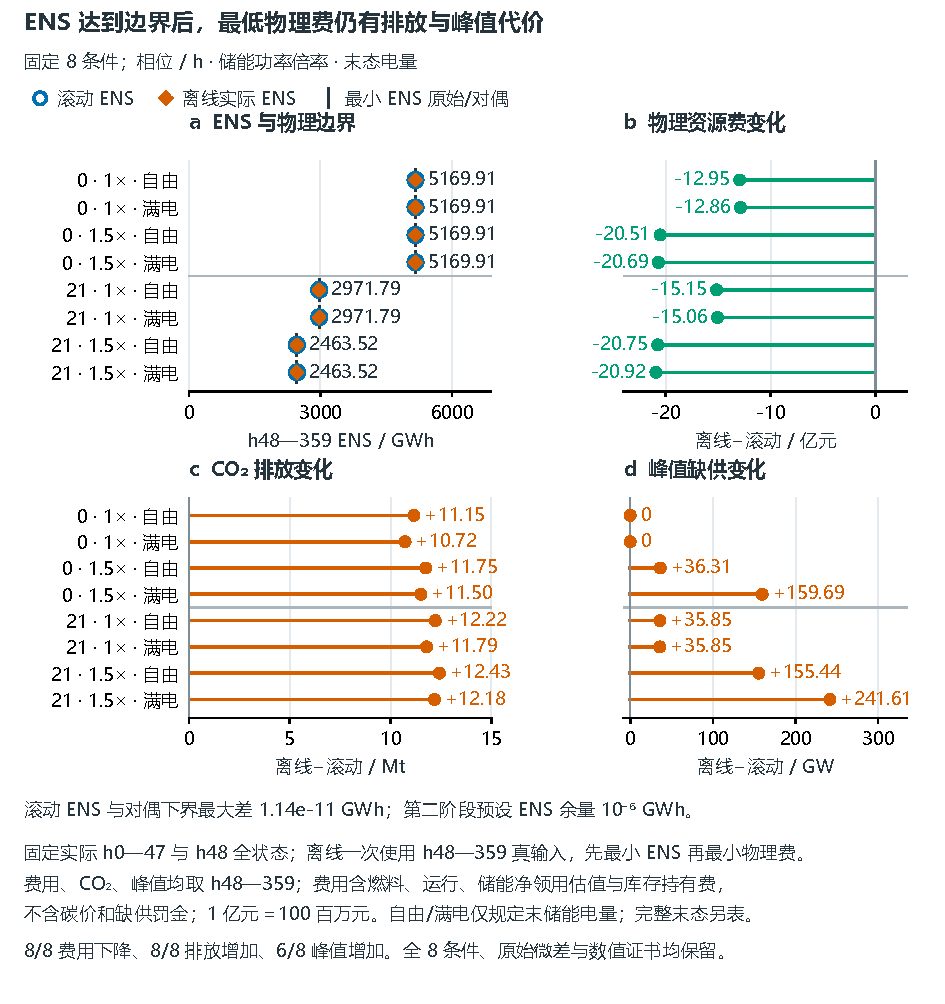
\includegraphics[width=160mm]{figures/figQ_dispatch_bound_tradeoffs.pdf}
\caption{固定前缀下的八组离线参照：累计缺供边界、物理资源费、排放及峰值。二阶段允许$10^{-6}$ GWh缺供容差；此图保留当次求解器选出的最优解；六条峰值升高均另有等费保峰替代，见正文联合约束图。原值与完整末态见配对表。}\end{figure}

\begin{table}[H]\centering\caption{原相位四个夜间窗口的守恒电量下界}
\begin{tabular}{rrrr}\toprule
全局小时h & \shortstack{可用发电后缺口\\GWh} & \shortstack{储能最大交付\\GWh} & \shortstack{ENS下界\\GWh}\\\midrule
65—71 & 2328.016 & 740.879 & 1587.137 \\
89—95 & 1680.148 & 740.879 & 939.268 \\
209—215 & 2306.845 & 740.879 & 1565.966 \\
233—239 & 1818.419 & 740.879 & 1077.539 \\
\bottomrule\end{tabular}
\smallskip\par\noindent 各窗结束于原24小时债务截止点；按七种电源可用出力计算，各储能允许从满电开始。
\end{table}\section{联合约束、数值表示与完整状态记录}
联合约束24案完整成功。附加同末态原16案保留12成功与4个求解器状态2；关闭预处理的8次诊断保留2成功与6个状态2。末态等式改写为同值固定界的最后8次另列独立身份，全部实际状态见完整状态表；成功解同时核对原矩阵KKT与360小时物理转移。算法诊断不计为独立工程条件。两法按SciPy 1.15.3官方接口设置，实际选项与环境保存在冻结协议中\cite{scipy_highs_1153}。

\begin{table}[H]\centering\caption{同末态固定队列的完整原始求解状态}
\begin{tabular}{llccccc}\toprule
\shortstack{相位/功率/\\末SOC} & 参考 & 原表示 & DS & IPM & \shortstack{等价\\DS} & \shortstack{等价\\IPM}\\\midrule
0/1/自由 & 无碳帽 & 成功 & — & — & — & — \\
0/1/自由 & 碳封顶 & 状态2 & 状态2 & 状态2 & 状态2 & 状态2 \\
0/1/满电 & 无碳帽 & 成功 & — & — & — & — \\
0/1/满电 & 碳封顶 & 状态2 & 成功 & 状态2 & 状态2 & 状态2 \\
0/1.5/自由 & 无碳帽 & 成功 & — & — & — & — \\
0/1.5/自由 & 碳封顶 & 状态2 & 状态2 & 成功 & 成功 & 状态2 \\
0/1.5/满电 & 无碳帽 & 成功 & — & — & — & — \\
0/1.5/满电 & 碳封顶 & 状态2 & 状态2 & 状态2 & 状态2 & 成功 \\
21/1/自由 & 无碳帽 & 成功 & — & — & — & — \\
21/1/自由 & 碳封顶 & 成功 & — & — & — & — \\
21/1/满电 & 无碳帽 & 成功 & — & — & — & — \\
21/1/满电 & 碳封顶 & 成功 & — & — & — & — \\
21/1.5/自由 & 无碳帽 & 成功 & — & — & — & — \\
21/1.5/自由 & 碳封顶 & 成功 & — & — & — & — \\
21/1.5/满电 & 无碳帽 & 成功 & — & — & — & — \\
21/1.5/满电 & 碳封顶 & 成功 & — & — & — & — \\
\bottomrule\end{tabular}
\smallskip\par\noindent DS为双单纯形，IPM为内点法；两轮诊断均关闭预处理。破折号表示该条件未列入该轮固定四案，不是求解失败。状态2保留求解器原返回值，不能单独作为物理不可行证明。算法不计为独立工程条件。
\end{table}
\begin{table}[H]\centering\caption{四个原参考向量的完整零求解见证检查}
\begin{tabular}{llr}\toprule
相位/功率/末SOC & 原域见证 & 峰值减上界/GW\\\midrule
0/1/自由 & 有效 & 0.000000 \\
0/1/满电 & 有效 & 0.000000 \\
0/1.5/自由 & 峰值超界 & 36.314724 \\
0/1.5/满电 & 峰值超界 & 112.849882 \\
\bottomrule\end{tabular}
\smallskip\par\noindent 四个参考全部检查，保留两个超界负项。原功率自由/满SOC参考通过原域KKT与既有360小时物理来源核对；其中自由案补齐最后一种见证。原参考全部沿用已保存轨迹，新增LP与新增物理小时均为零。
\end{table}
固定末库存还揭示约束结构。对同一到货与直接服务路径，燃料总领用$Q_f=S_{f,48}+\sum I_{f,t}-S_{f,360}$，因此$C=\sum_f\epsilon_fQ_f$随三燃料末库存确定。独立代数核查将936条燃料余额等式按原排放系数加权并扣除三条末库存等式，所得系数与碳上界行的最大差为$1.09\times10^{-19}$，RHS差为$6.54$—$7.56\times10^{-12}$ Mt。该冗余与两方法分歧一并保留，不以单次状态2判定物理域为空。

\noindent 关键逐行结果见\path{outputs/v16/joint_dispatch_figures/}；八组工程条件、原16案和两轮诊断的全部失败均保留。\par

\section{结果标识与精确参数}
方案Ⅰ、Ⅱ、Ⅲ分别对应程序标识005、006、007。第21号联合设计的GDP增速倍率为1.186736，资本倍率为0.782592，进口倍率为0.760028。全部建设机制差值以图中明确的P0参照报告，原48组、32事件格与全部八组约束比较的原值均保留在支撑材料。表内舍入值用于阅读，精确值以对应原始计算表为准。

官方附件处理入口为\path{src/v17_station_evidence.py}，本版图件入口为\path{src/v18_main_visuals.py}和\path{src/v18_evidence_visuals.py}；论文稿源位于\texttt{paper/V18成果稿/}。
